\chapter{蒙特卡洛方法}
\label{chap:17}
%%%%%%%%%%%%%%%%%%%%%%%%%%%%%%%%%%%%%%%%%%%%%%%%%%%%%%%%%
%%%%%%%%%%%%%%%%%%% author:kiseliu  %%%%%%%%%%%%%%%%%%%%%
%%%%%%%%%%%%%%%%%%% part17.0-17.3   %%%%%%%%%%%%%%%%%%%%%
%%%%%%%%%%%%%%%%%%%%%%%%%%%%%%%%%%%%%%%%%%%%%%%%%%%%%%%%%


随机化算法可以分成大致两类:拉斯维加斯算法和蒙特卡罗算法。拉斯维加斯算法总是准确地返回正确答案(或者报告失败)。这类算法使用随机数量的资源,通常是内存或者时间。相反,蒙特卡罗算法返回答案时会带有随机量的错误。错误量通常可以通过扩展更多的资源(通常是运行时间和内存)被减少。对任意固定的计算方案,蒙特卡罗都可以给出一个近似回答。

机器学习领域中的许多问题都很困难,除了精确的确定性算法和拉斯维加斯算法,我们不能期待获得这些困难问题的精确答案。相反,我们必须使用确定性的近似算法或者蒙特卡罗近似,这两种方法在机器学习中是广泛存在的。本章,我们将讨论蒙特卡罗方法。

\section{采样和蒙特卡罗方法}
许多用于实现机器学习目标的重要技术都是基于从一些概率分布中抽取样本,然后用这些样本进行一定理想数量的蒙特卡罗估计。

\subsection{为什么采样?}
我们想要从概率分布中抽取样本有许多原因。采样用更少的代价,提供了一种灵活的方法来近似许多加和和积分。有时候我们使用采样来加速代价昂贵但是容易处理的加和,比如我们使用minibatches获得对整个训练代价重采样的情况。在其他情况,我们的学习算法需要逼近一个不容易处理的加和或者积分,比如对数模型的对数配分函数(log partition function)的梯度。在许多其他情况下,在我们想训练一个其数据来自于训练分布的模型的意义上,采样确实是我们的目标。


\subsection{蒙特卡罗采样的基本知识}
 当加和或者积分不能准确地被计算出来(比如,该加和具有指数级别数量的项,并且没有精确的简化),我们经常会使用蒙特卡罗采样来逼近它。其思想是将加和或者积分看作是某种分布下的期望,然后通过相应的平均来近似该期望。令
 $$ s = \sum _{ x }^{  }{ p(\bm{x})f(\bm{x}) ={ E }_{ p }[f(\textbf{x})] }\eqno{(17.1)} $$
或者
 $$ s=\int { p(\bm{x})f(\bm{x})d\bm{x}= } { E }_{ p }[f(\textbf{x})]\eqno{(17.2)} $$
 是将要估计的加和或者积分,我们把它重新写成一个期望,这里$p$是随机变量\(\textbf{x}\)的概率分布(对加和而言)或者概率密度(对积分而言)。

 我们可以通过从$p$中抽取$n$个样本 $ { \bm{x} }^{ (1) },...,{ \bm{x} }^{ (n) }$,然后构建下面的经验平均来估计$s$:
 $${ \hat { s }  }_{ n } =\frac { 1 }{ n } \sum _{ i=1 }^{ n }{ f({ \bm{x} }^{ (i) }) } .\eqno{(17.3)}$$
这种近似可以由几个不同的性质来证明。首先,我们通过观察可以发现\(\hat { { s } } \)是无偏的,因此
$$\mathbb{E}[\hat{s}_n]=\frac{1}{n}\sum_{i=1}^{n}\mathbb{E}[f(\bm{x}^{(i)})]=\frac{1}{n}\sum_{i=1}^{n}s=s .\eqno{(17.4)}$$
但是除此之外,大数定律告诉我们如果样本\({ \bm{x} }^{ (i) }\)是独立同分布,那么几乎可以肯定该平均收敛于期望值:
$$\lim _{ n\rightarrow \infty  }{ { \hat { s }  }_{ n }= } s, \eqno{(17.5)}$$
上式成立的条件是每一项的方差\(Var[f({ \bm{x} }^{ (i) })]\)是有界的。为了看的更清楚,考虑\(n\)递增时\({\hat { s }  }_{ n }\)的方差。只要
\(Var[f({ \textbf{x} }^{ (i) })]<\infty \),方差\(\text{Var}[{ \hat { s }  }_{ n }]\)递减且收敛于0:
$$ \text{Var}[{ \hat { s } }_{ n }]=\frac { 1 }{ { n }^{ 2 } } \sum _{ i=1 }^{ n }{ \text{Var}[f(\textbf{x})] }  \eqno{(17.6)}$$
$$=\frac { \text{Var}[f(\textbf{x})] }{ n } . \eqno{(17.7)}$$
这个简便的结论也告诉了我们如何用蒙特卡罗平均估计不确定或者等价地蒙特卡罗近似的预期误差量。我们计算\(f({\bm{x}}^{ (i) })\)的经验平均\footnote{更常说方差的无偏估计量,其中平方误差和除以n-1而不是n。}和经验方差,然后用样本数量\(n\)来除估计的方差获得\(\text{Var}[{\hat { s }  }_{ n }]\)的估计。中心极限定理告诉我们分布的均值\({\hat { s }  }_{ n }\)收敛到均值为\(s\),方差为\(\frac { \text{Var}[f(\bf{x})] }{ n } \)的正态分布。这使得我们能够使用正态密度的累计分布来估计\({\hat { s }  }_{ n }\)的置信区间。

然而所有这些依赖于我们能否很容易地从基本分布\(p(\bf{x})\)进行采样,但是我们可能并不能总是这样做。如果从\(p\)中采样不合理时,另一种方法是使用重要性采样,我们会在\textcolor{red}{17.2}节介绍它。一种更常用的方法是构造收敛到感兴趣的分布的估计序列,这种方法是蒙特卡罗马尔可夫链(见\textcolor{red}{17.3}节)。


\section{重要性采样}

在方程17.2中,蒙特卡罗方法使用的被积函数(或被加数)分解中,有一步很重要,那就是决定被积函数的哪部分应该作为概率分布\(p(\bm{x})\),被积函数的哪部分应该作为其期望值(在概率分布下)被估计的数量函数\(f(\bm{x})\)。由于\(p(\bm{x})f(\bm{x})\)总是可以被写成
$$p(\bm{x})f(\bm{x})=q(\bm{x})\frac { p(\bm{x})f(\bm{x}) }{ q(\bm{x}) } ,\eqno{(17.8)}$$
所以被积函数没有唯一的分解。这里我们从\(q\)和均值\(\frac{pf}{q}\)进行抽样。在许多情况下,我们希望对于给定的\(p\)和\(f\)计算期望,并且从开始指定问题作为期望的事实表明这个\(p\)和\(f\)将是一种自然分解。但是就为了得到给定精度的准确率所需要的样本数量而言,问题的原始规范形式可能并不是最优的选择。幸运地是,最优选择\({ q }^{ * }\)的形式可以很容易地被推导出来。最优的\({ q }^{ * }\)对应于最优的重要性采样。

由于方程17.8中等式,任何蒙特卡罗估计:
$${ \hat { s }  }_{ p }=\frac { 1 }{ n } \sum _{ i=1,{ \bf{x} }^{ (i) }\sim  p }^{ n }{ f({ \bm{x} }^{ (i) }) } \eqno{(17.9)}$$
都可以被转换为重要性采样估计:
$${ \hat { s }  }_{ q }=\frac { 1 }{ n } \sum _{ i=1,{ \bf{x}}^{ (i) } \sim  q }^{ n }{ \frac { p({\bm{x}}^{ (i) })f({\bm{x}}^{ (i) }) }{ q({\bm{x}}^{ (i) }) }  } . \eqno{(17.10)}$$

我们可以很容易地看到估计的期望值不依赖于\(q\):
$$\mathbb{E}_{ q }\left[ \hat { { s }_{ q } }  \right] =\mathbb{E}_{ q }\left[ \hat { { s }_{ p } }  \right] =s. \eqno{(17.11)}$$
但是,重要性采样估计的方差对\(q\)的选择非常敏感。方差由下式给出:
$$\text{Var}[\hat { { s }_{ q } } ]=\text{Var}[\frac { p(\bf{x})f(\bf{x}) }{ q(\bf{x}) } ]/n. \eqno{(17.12)}$$
当\(q\)取值如下的时候,可以使得方差最小:
$${ q }^{ * }(\bm{x})=\frac { p(\bm{x})|f(\bm{x})| }{ Z } , \eqno{(17.13)}$$
这里Z是正则化常数,它被用来使得\({ q }^{ * }(\bm{x})\)加和或者积分等于1。越好的重要性采样分布,在被积函数越大的地方,赋予的权重就越大。事实上,当\(f(\bm{x})\)不改变符号,\(\text{Var}[{ \hat { s }  }_{ { q }^{ * } }]=0\),这意味着当我们使用最优分布时,单样本就足够了。当然,这只是因为\(q^{*}\)的计算基本上解决了原始问题,从最优分布中抽取一个单样本通常是不切实际的。
(从获得正确期望值的意义上来说)采样分布\(q\)的任何选择都是有效的,并且(从获得最小方差的意义上来说)\(q^{*}\)是最优的一个。从\(q^{*}\)中采样通常是不可行的,但是当我们继续减少方差,\(q\)的其他选择是可行的。

另一种方法是使用有偏的重要性采样,它的一个优势是不需要正则化的\(p\)或者\(q\)。在离散变量的情况下,有偏的重要性采样估计由下式给出:
$${ \hat { s }  }_{ BIS }=\frac { \sum _{ i=1 }^{ n }{ \frac { p({\bm{x}}^{ (i) }) }{ q({\bm{x}}^{ (i) }) }  } f({\bm{x}}^{ (i) }) }{ \sum _{ i=1 }^{ n }{ \frac { p({\bm{x}}^{ (i) }) }{ q({\bm{x}}^{ (i) }) }  }  } \eqno{(17.14)}$$
$$=\frac { \sum _{ i=1 }^{ n }{ \frac { p({\bm{x}}^{ (i) }) }{ \tilde { q } ({\bm{x}}^{ (i) }) }  } f({\bm{x}}^{ (i) }) }{ \sum _{ i=1 }^{ n }{ \frac { p({\bm{x}}^{ (i) }) }{ \tilde { q } ({\bm{x}}^{ (i) }) }  }  } \eqno{(17.15)}$$
$$=\frac { \sum _{ i=1 }^{ n }{ \frac { \tilde{p}({\bm{x}}^{ (i) }) }{ \tilde { q } ({\bm{x}}^{ (i) }) }  } f({\bm{x}}^{ (i) }) }{ \sum _{ i=1 }^{ n }{ \frac {\tilde {p}({\bm{x}}^{ (i) }) }{ \tilde { q } ({\bm{x}}^{ (i) }) }  }  }, \eqno{(17.16)}$$
这里\(\tilde {p}\)和\(\tilde {q}\)是\(p\)和\(q\)的无正则化形式,\({\bm{x}}^{ (i) }\)是\(q\)中的样本。除了\( n\rightarrow \infty\)和方程17.14的分母收敛于1的情况,该估计是有偏的,因为\(\mathbb{E}\left[ \hat { { s }_{ BIS } }  \right] \neq s\)。因此这种估计被叫做渐进无偏的。

尽管\(q\)的一个好的选择可以极大地提高蒙特卡罗估计的效率,但是一个不好的选择会使得效率更差。回到方程17.12,我们可以看到如果\( \frac { p(\bm{x})|f(\bm{x})| }{ q(\bm{x}) } \)中的\(q\)的样本很大,那么估计的方差会变得非常大。这可能发生在\(q(\bm{x})\)很小,而\(p(\bm{x})\)和\(f(\bm{x})\)都不够小来抵消它时。\(q\)分布通常被选择为非常简单的分布以使得容易进行抽样。当\(\bm{x}\)是高维的,\(q\)的简单性会使得它对\(p\)或者\(p|f|\)的匹配非常糟糕。当\(q({\bm{x}}^{ (i) })\gg p({\bm{x}}^{ (i) })|f({\bm{x}}^{ (i) })\)|,重要性采样会得到一些无用的样本(总和微小的数字或零)。另一方面,当\(q({\bm{x}}^{ (i) })\ll p({\bm{x}}^{ (i) })|f({\bm{x}}^{ (i) })\)|,尽管这种情况更少发生,但是无用的样本比例会很大。由于后者的情况是极少的,它们可能不会出现在典型的样本中,产生s的典型低估,很少被大量过高估计补偿。所谓典型的,当\(\bm{x}\)是高维的,非常大或者非常小的数字就是典型的,因为在高维情况下,联合概率的动态范围是非常大的。

尽管存在上述危险,但是重要性采样和它的变种们在许多机器学习算法中都非常有用,包括深度学习算法。比如,使用重要性采样可以加速具有很大词汇表的神经语言模型(\textcolor{red}{12.4.3.3}章节),或者具有很多输出的其他神经网络的训练。另请参考\textcolor{red}{18.7}章节重要性采样是如何被用来估计配分函数(概率分布的正则化常数)的,和\textcolor{red}{20.10.3}章节重要性采样是如何被用来估计深度有向模型,比如变分自编码器的对数似然的。重要性采样可以被用来改进代价函数的梯度估计,该代价函数被用来训练使用随机梯度下降的模型的参数,特别是对于诸如分类器的模型,其中代价函数的大部分总值来自很少量的被分错的样本。更频繁地抽样更困难的例子可以减少这种情况下梯度的方差(Hinton,2006)。

\section{马尔可夫蒙特卡罗方法}
在许多情况下,我们想要使用蒙特卡罗技术,但是没有容易的方法从分布\({ p }_{ model }(\bf{x})\)或者从一个好的(低方差)重要性采样分布\(q(\bf{x})\)中抽取精确的样本。在深度学习中,这种情况经常发生在\({ p }_{ model }(\bf{x})\)被一个无向模型表示时。在这些情况下,我们引入一种数学工具叫马尔可夫链来近似地从\({ p }_{ model }(\bf{x})\)中采样。使用马尔可夫链来进行蒙特卡罗估计的一类算法叫做马尔可夫蒙特卡罗方法(MCMC)。在Koller and Friedman (2009)中,用了很大篇幅来描述机器学习中的马尔可夫蒙特卡罗方法。
MCMC技术最标准且通用的保证仅适用于模型不对任何状态指定零概率的情况。因此,把这些技术表示成从如在\textcolor{red}{16.2.4}中描述的基于能量的模型(EBM) \(p(\bm{x})\propto \text{exp}(-E(\bm{x}))\)中采样是最方便的。在EBM公式中,每个状态都被确保具有非零概率。实际上,MCMC方法具有更广泛的适用性,并且可以被与包含零概率状态的许多概率分布一起使用。但是,关于MCMC方法表现的理论保证必须在不同类型的分布下逐个证明。在深度学习的背景下,依赖于能够应用所有基于能量的模型的最一般的理论保证是最常见的。

为了理解为什么从基于能量的模型抽取样本是困难的,让我们考虑只有两个变量的EBM模型,定义一个分布\(p(\text{a,b})\)。为了采样\(\text{a}\),我们必须从\(p(\text{a|b})\)中抽取\(\text{a}\),为了采样\(\text{b}\),我们必须从\(p(\text{b|a})\)中抽取\(\text{b}\)。它看起来是个不容易处理的鸡生蛋,蛋生鸡的问题。有向模型可以避免这个问题,因为它们的图是有向无环的。要进行祖先采样,只需要按照拓扑顺序对每个变量进行采样,对每个变量的父节点进行调节,并保证父节点已经被采样(见第\textcolor{red}{16.3}节)。祖先采样定义了一种获得样本的有效的单程方法。

在EBM模型中,我们可以通过使用马尔可夫链来抽样,从而避免这个鸡生蛋,蛋生鸡的问题。马尔可夫链的核心思想是有一个以任意值开始的状态,随着时间,我们不断地随机更新\(\bm{x}\)。最终\(\bm{x}\)(几乎接近)变成\(p(\bm{x})\)中的一个真实的样本。正式来说,马尔可夫链被定义为随机状态\(\bm{x}\),和转移分布\(T({ \bm{x} }^{ \prime  }|\bm{x})\),该分布给出了从状态\(\bm{x}\)开始,随机更新到状态\({ \bm{x} }^{ \prime  }\)的概率。运行马尔可夫链意味着不断地更新状态\(\bm{x}\)到从\(T({ \bf{x} }^{ \prime  }|\bm{x})\)抽样出来的值\({ \bm{x} }^{ \prime }\)。

为了得到一些关于MCMC方法如何工作的理论理解,对其进行再参数化是很有用的。首先,我们把问题限制在随机变量\(\bf{x}\)只有有限种状态的情况。在这种情况,我们可以把状态表示成一个正整数\(x\)。$x$的不同的整数值对应原始问题中不同的状态\(\bm{x}\)。

现在让我们考虑下,当我们无限次并行地运行许多马尔可夫链时会发生什么。不同的马尔可夫链的所有状态都是从相同的分布\({ q }^{ (t) }(x)\) 中抽取的,这里\(t\)表示已经过去的时间步长的数量。在开始时,\({ q }^{ (0) }\)是一些用来对每个马尔可夫链任意地初始化\(x\)的分布。随后,\({ q }^{ (t) }\)被目前已经运行过的所有的马尔可夫链步骤所影响。我们的目标是让\({ q }^{ (t) }(x)\)收敛到\(p(x)\)。

因为我们已经就正整数\(x\)重新参数化了该问题,因为我们可以用一个向量\(\bm{v}\)来描述概率分布\(q\),如下式:
 $$ { q }(\text{x}=i)={ v }_{ i }. \eqno{(17.17)} $$

 考虑下当我们更新单独一个马尔可夫链的状态\(x\)到一个新的状态\({x}^{\prime}\)时,会发生什么。一个单独的状态落到状态\({x}^{\prime}\)的概率由下式给出:
$${ q }^{ (t+1) }({ x }^{ \prime  })=\sum _{ x }^{  }{ { q }^{ (t) }({ x }) } T({ x }^{ \prime  }|x).  \eqno{(17.18)}  $$

使用我们的整数参数化,我们可以用矩阵\(\bm{A}\)表示转移操作\(T\)的影响。我们定义\(\bm{A}\)为:
$${ A }_{ i,j }=T({ \bf{x} }^{ \prime  }=i|{\bf{x}} = j). \eqno{(17.19)}  $$

使用这个定义,我们现在可以重写方程17.18。代替书写该公式使用\(q\)和\(T\)来理解单个状态是如何被更新的,我们可能可以用\(\bm{v}\)和\(\bm{A}\)把基于所有不同马尔可夫链的整个分布是如何并行运行的过程描述为我们进行的一次更新:
$${\bm{v}}^{ (t) }=\bm{A}{\bm{v}}^{ (t-1) }. \eqno{(17.20)}$$

应用马尔可夫链不断地进行更新,对应于不断地乘以矩阵\(\bm{A}\)。也就是说,我们可以把该过程看作对矩阵\(\bm{A}\)取幂:
$${ \bm{v} }^{ (t) }=\bm{A}{ \bm{v} }^{ (0) }.  \eqno{(17.21)}$$

矩阵\(\bm{A}\)有特殊的结构,它的每一列表示一个概率分布。这样的矩阵也叫做随机矩阵。如果在某次幂\(t\),从任意状态\(x\)转移到其他状态\({x}^{ \prime }\)的概率都非零,那么Perron-Frobenius定理(Perron, 1907; Frobenius, 1908)保证,最大的特征值是实数,并且等于1。随着时间,我们可以看到所有的特征值都可以写成指数形式:
$${\bm{v}}^{(t)}={(\bm{V}diag(\bm{\lambda}){\bm{V}}^{-1})}^{t}{\bm{v}}^{(0) }=\bm{V}diag(\bm{\lambda})^t{\bm{V}}^{ -1 }{\bm{v}}^{ (0) } \eqno{(17.22)}$$

该过程会使得所有不等于1的特征值衰减到0。在其他宽松的条件下,A被确保只有一个特征值为1的特征向量。因此该过程收敛到稳定分布,有时也称为平衡分布。收敛时,
$${ \bm{v} }^{ \prime  }=\bm{A}\bm{v}=\bm{v}, \eqno{(17.23)}$$
这个相同的条件对每个额外的步骤都成立。这是一个特征向量方程。为了成为一个稳定点,\(\bm{v}\)必须是对应于特征值为1的特征向量。这个条件确保一旦到达稳定分布,转移抽样过程的重复应用不改变基于各种各样的马尔可夫链的状态的分布(尽管转移操作本来就不改变每个个体状态)。

如果我们正确地选择了\(T\),那么稳定分布\(q\)会等于我们希望抽样的分布\(p\)。我们会在\textcolor{red}{17.4}章节简要地描述如何选择\(T\)。

具有可数状态的马尔可夫链的大多数性质可以推广到连续变量的马尔可夫链。在这种情况下,一些作者称马尔可夫链为Harris链,但是我们使用马尔可夫链这个术语来描述这两种情况。通常在宽松的条件下,具有转移操作\(T\)的马尔可夫链会收敛到一个稳定点,该点可以用下述方程来描述:
$$  {q}^{\prime}(\bf{x}^{\prime})={\mathbb{E}}_{\bf{x}\sim q}T(\bf{x}^{\prime}|\bf{x})  \eqno{(17.24)} $$
 离散的情况,我们刚才已经重写成方程17.23了。当\(\bf{x}\)是离散的,期望对应于加和,当\(\bf{x}\)是连续的,期望对应于积分。

不管状态是连续的还是离散的,所有的马尔可夫链方法都包含重复地应用随机更新的过程,直到最终状态开始从平稳分布产生样本。运行马尔可夫链直到它达到平稳分布的过程叫做“burning in”马尔可夫链。在达到了平稳分布,非常多的样本序列可以从平稳分布中抽取出来。它们被相同地分布,但是任意两个成功的样本之间是高度相关的。因此有限的样本序列可能不能表示平稳分布。减轻这个问题的一种方法是仅返回每\(n\)个连续样本,这会使得我们对平衡分布的统计的估计不会由于MCMC采样和接下来的几个样本之间的相关性而有偏差。因此使用马尔可夫链的代价很高,因为需要时间来构建平稳分布,以及在达到平稳后需要时间从一个样本转换到另一个合理地去除了相关性的样本。如果想得到真正独立的样本,可以并行地运行多个马尔可夫链。这种方法使用了额外的并行代价来消除延迟。只使用一个单独的马尔可夫链来产生所有的样本的策略,和对每一个理想的样本都使用一个马尔可夫链的策略是两种极端;深度学习从业人员通常使用与小批量中的样本数量相似的多个链,然后从这个固定的马尔科夫链中绘制所需的多个样本。常用的马尔可夫链的数目是100。

另一个困难是我们不能提前知道,在达到平稳分布前,马尔可夫链要运行多少步。该时间长度称为混合时间。测试马尔可夫链是否达到平衡也是非常困难的。暂时没有足够准确的理论来指导我们回答这一问题。理论只是告诉我们,马尔可夫链会收敛,没有更多的信息了。如果我们从作用于概率向量\(\bm{v}\)的矩阵\(\bm{A}\)的角度来分析马尔可夫链,那么我们知道当\({ \bm{A} }^{ t }\)已经有效地丢失了来自\(\bm{A}\)的除了唯一的特征值1之外的所有特征值时,链条混合。这意味着第二大的特征值的量级将决定混合时间。但是实际上,我们不能用矩阵表示出马尔可夫链。我们的概率模型可以访问的状态数量对于变量的数量是指数级大的,所以表示\(\bm{v}\),\(\bm{A}\)或者\(\bm{A}\)的特征值是不合理的。由于这些阻碍和其他的阻碍,我们通常不知道马尔可夫链是否已经混合。相反,我们简单地运行马尔可夫链一段时间,然后大致地估计是否足够,并且使用启发式方法来确定链是否混合。这些启发式方法包括人工检查样本,或者测量成功抽取的样本之间的相关性。


\section{吉布斯采样}
\label{sec:17.4}

到目前为止,本章已经介绍了如何通过迭代更新$\bm{x}\leftarrow \bm{x}' \sim T (\bm{x}'|\bm{x}) $在概率分布$q(\bm{x})$上采样的方法.
但是,还没有说明怎样确保$q(\bm{x})$是有效的概率分布.
本书主要考虑两种基本方法.第一种方法根据给定的通过学习得到的$p_{model}$推导出$T$,下文将会详细介绍从EBMs(energy-based model)采样的例子.
第二种方法是直接参数化$T$并学习,使其平稳分布可以隐式地定义$p_{model}$的兴趣点.
第二种方法的例子将在章节"\textcolor{red}{20.12}"和"\textcolor{red}{20.13}"阐述.

在深度学习中,通常使用马尔科夫链从以基于能量的模型定义的概率分布$p_{model}(\bm{x})$中采样.
此例中,马尔科夫链所需的$q(\bm{x})$就是$p_{model}$.
为得到满足需求的$q(\bm{x})$,必须选择合适的$T(\bm{x}'|\bm{x})$.

为了构建马尔科夫链,一种概念上简单有效的方法就是使用\textit{吉布斯采样}从$p_{model}(\bm{x})$中采样.
在吉布斯采样中,通过选择一个变量$\textbf{x}_i$实现从$T(\textbf{x}'|\textbf{x})$中采样,$\textbf{x}_i$的选择方法取决于它在基于能量模型结构的无向图$\mathcal{G}$上的邻居变量.
只要给定的所有邻居节点都条件独立,也可以同时对多个变量采样.
在\textcolor{red}{16.7.1}中的RBM(受限玻尔兹曼机)例子中,RBM的所有隐含层单元可以被同时采样,是因为他们都条件独立于其他的给定可视层单元.
同样的,因为对于给定的隐含层单元,所有的可视层单元都是条件独立的,因此所有的可视层单元也可以同时被采样.
以这种方式同时更新多个变量的吉布斯采样方法,被称为块吉布斯(block gibbs)采样.

从$p_{model}$中采样来设计马尔科夫链的代替方法是可行的.例如,Metropolis-Hastings算法就广泛应用于其他学科领域.
在深度学习领域实现无向建模,除吉布斯采样外很少使用其他方法.
改进采样技术是一个潜在的研究领域.

\section{分离状态混合的挑战}
\label{sec:17.5}

$MCMC$方法的主要问题是混合效果比较差.理想情况下,从$p(\bm{x})$分布设计的马尔科夫链中得到连续采样之间将会是完全相互独立的,
这些采样在$\bm{x}$空间下访问不同的区域可能性与他们的概率成正比.
然而,尤其是在高维情况下,MCMC样本之间会强相关.
我们称这种行为是缓慢混合,甚至是失败混合.
相对于链(随机变量被采样)的状态,$MCMC$方法的缓慢混合可以被看作是在能量函数上随意地执行了类似嘈杂梯度下降(noisy gradient descent)操作,
或者等效地在概率函数上执行嘈杂爬山(noisy hill climbing)操作.
马尔科夫链往往使用渐进策略(在马尔科夫链状态空间中),从组态$\bm{x}_{(t-1)}$到$\bm{x}_{(t)}$,
能量$E(\bm{x}_{(t)})$往往低于或约等于能量$E(\bm{x}_{(t-1)})$,偏好会产生较低能量组态的移动.
当从相对不可能的组态(比来自$p(\textbf{x})$的典型构型具有更高的能量)开始时,链趋向于逐步降低能量的状态仅仅偶尔移动到另一种状态.
一旦链找到了低能量的区域(例如,假设变量是图片中的像素点,则低能量的区域可以是同一对象的图像中的连通的多边形),我们称其之为一个状态,链将会尝试在状态上游走(类似于随机游走).
一旦跳出那个状态,一般会返回原状态或者(如果找到了逃离路线)会移动到另一个状态.
问题是成功的逃离路线很少有很多有趣的分布,所以马尔科夫链将会在同一状态而不是它应有的状态上连续采样.

在使用吉布斯采样算法时这一点是显而易见的(章节\textcolor{red}{17.4}).
在这种情况下,在特定的步骤内从一个状态转移到邻近状态的概率取决于状态之间"能量势垒"(energy barrier)的形状.
被高能量势垒(低概率区域)分隔的两个状态之间是不太可能发生转移的(在能量势垒的高度方面).
如图$17.1$所示.
当多个高概率状态被低概率区域分隔时会出现问题,特别是当吉布斯采样每步仅仅更新一小部分变量,而这部分变量的值主要由其它变量确定时.

举个简单的例子,假设基于能量模型的两个变量$\text{a}$和$\text{b}$,他们是带符号的二进制,取值为-1和1.
对于模型$E(\text{a,b})=-w\text{ab}$,如果$w$是一个大正数,那么这个模型中的$\text{a}$和$\text{b}$极有可能具有相同的符号.
如果使用$\text{a}=1$的吉布斯采样步骤来更新$\text{b}$,那么$\text{b}$的条件分布则是由$P(\text{b}=1|\text{a}=1)=\sigma(w)$确定的.
如果$w$很大,$\text{b}$也赋值为1的概率接近于1.
同理,如果$\text{a}=-1$,则将$\text{b}$赋值为-1的概率接近1.
根据$P_{model}(\text{a},\text{b})$模型,两个变量的符号可能相同.
也就是说,吉布斯采样不会改变变量的符号.

实际应用场景更具有挑战性,因为不仅要关注两个状态之间的转移,而且在更具一般性的真实模型中可能更关心多个状态之间的转移.因为状态混合困难性,获取覆盖大多数状态的可靠样本集合花费的代价巨大,而且由于到达马尔科夫链稳定分布状态的收敛速度非常慢等诸多原因,这样的多个状态之间的转移是很难的.

有时这个问题可以通过找到含有高度依赖性单元的群体并按块同时更新所有这些单元来解决.
然而不幸的是,这种依赖性是复杂的,从这样的群体中采样是难以计算的.
毕竟,马尔科夫链最初被引入来解决的问题就是怎样从一组变量中采样.

\begin{figure}[htbp]
	\centering
	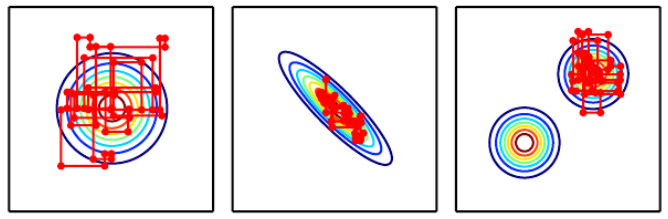
\includegraphics[width=5in]{fig/chap17/chap17.1.png}
	\caption{三种分布的吉布斯采样路径,在这两种情况下,马尔科夫链以同样的模式初始化.
	$($左图$)$两个条件独立变量的多变量正态分布.因为变量之间是条件独立的,所以吉布斯采样混合的很好.
	$($中图$)$变量高度相关的多变量正态分布.变量之间的相关性使得马尔科夫链很难混合.因为每个变量的更新都要取决于其他变量,相关性降低了马尔科夫链从起始点移动到其他状态的概率.
	$($右图$)$广泛分离模式的高斯分布的混合是非轴对称的.因为当一次仅改变一个变量时,马尔科夫链难以改变状态,所以吉布斯采样混合的很慢.}
	\label{fig:chap17.1.png}
\end{figure}

在含有隐含变量的模型中,定义了联合分布$p_{model}(\bm{x}|\bm{h})$,常常通过交替在$p_{model}(\bm{x}|\bm{h})$和$p_{model}(\bm{h}|\bm{x})$中对$\bm{x}$进行采样.
从快速混合的目的出发,我们希望$p_{model}(\bm{h}|\bm{x})$有更高的熵.
但是,从学习到有用的$\bm{h}$的表达式的目的出发,我们又希望$\bm{h}$有足够的信息来编码并重建$\bm{x}$,这意味着$\bm{h}$和$\bm{x}$应该有很高的交互信息.
这个两个目标是相互矛盾的.
常见的生成模型可以非常精确地将$\bm{x}$编码为$\bm{h}$,但是往往不能混合地很好.
这种情况在玻尔兹曼机中很常见-玻尔兹曼机学习到的分布越尖锐,马尔科夫链从分布模型中的采样就越难以混合良好.
这个问题在图$17.2$中说明.

当兴趣分布具有多种结构且每一类有单独的样本,所有上述问题都可能导致$MCMC$方法在兴趣分布上失效:
概率分布集中在许多状态周围,这些状态被高能量区域分隔开.
这类分布就是我们在许多分类问题中期望的,状态之间的较差混合导致$MCMC$方法收敛地非常缓慢.

\begin{figure}[htbp]
	\centering
	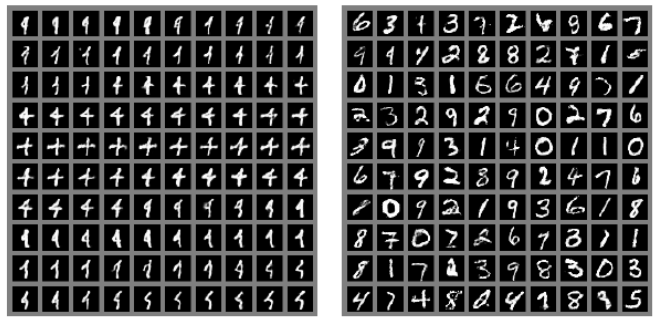
\includegraphics[width=5in]{fig/chap17/chap17.2.png}
	\caption{在深度概率模型中漫混合问题的例子.每个图像应该从左到右,从上到下阅读.
	$($左图$)$是来自吉布斯采样的连续样本应用于MNIST数据集上训练的深度玻尔兹曼机.连续样本之间是很相似的.
	因为吉布斯采样是在深度图模型中执行的,所以这种相似性更多地基于语义而不是原始视觉特征,
	但是吉布斯链仍然难以从分布的一种状态转换到另一种状态,例如通过改变数字标识.
	$($右图$)$是来自生成对抗网络的连续祖代样本.因为祖代采样独立于其他样本而生成每个样本,所以没有混合问题.}
	\label{fig:chap17.2.png}
\end{figure}

\section{17.5.1 基于回火的状态混合}
\label{sec:17.5.1}

当一个分布显示出的形态是低概率区域围绕着高概率的“尖峰”时候,这个分布的不同状态很难混合。很多快速混合技术都基于构建的可以替代目标分布的版本,在新构建的分布中峰没有目标分布高,周围的谷也没有目标分布低。基于能量的模型提供了一个特别简单的方法来实现。到目前为止,我们已经描述了一个基于能量的模型来作为概率分布的定义,如下式:

$$p(\bm{x})\propto exp(-E(\bm{x})).  \eqno{(17.25)} $$

基于能量的模型可以增加一个额外的参数$\beta$来控制这个分布快速达到峰值:

$$p_{\beta}(\bm{x})\propto exp(-\beta E(\bm{x})).  \eqno{(17.26)}$$

参数$\beta$通常被描述为温度的倒数,这反映了基于能量的模型在统计物理学中的起源。当温度下降到零并且$\beta$趋于无穷大时,基于能量的模型变得稳定。当温度趋于无穷大并且$\beta$下降到零时,离散$\bm{x}$的分布变得均匀。

通常来说,可以训练一个模型来得到$\beta=1$时的估计值。然而,我们可以使用其他温度,特别是$\beta<1$处的温度。回火是通过描绘$\beta<1$的采样来实现$p_{1}$的多个状态之间快速混合的一个一般性策略。

为了混合不同的模式,基于回火转换的马尔可夫链(Neal在1994年提出)暂时从更高的温度分布采样,然后再恢复到从单位温度分布上采样。
这些技术已经被应用到一些模型上,比如RBMs(Salakhutdinov在2010年提出)。
另一种方法是使用并行回火(Iba在2001年提出),其中马尔可夫链在不同温度下,并行模拟了许多不同的状态。
最高温度状态下混合缓慢,但是最低温度状态在温度为1时提供了来自模型的精确样本。
转换操作包括在两种不同温度水平下随机切换状态,因此从高温时隙中获得的一个高概率样本可以跳到一个较低温度的时隙中。
这个方法也被应用到RBMs中(Desjardins等在2010年提出;Cho等在2010年提出)。
虽然回火是一种很有使用前景的方法,但是现在研究人员还没能在从复杂EBMs采样的问题上取得突破性进展。
一个可能的原因是为了使得回火有效临界温度周围的温度转换必须是非常缓慢的(因为温度是逐渐降低的)。

\section{17.5.2 深度会促进混合}
\label{sec:17.5.2}

当从一个隐变量模型$p(\bm{h},\bm{x})$采样时,我们看到,如果$p(\bm{h}|\bm{x})$对$\bm{x}$编码太长,则从$p(\bm{x}|\bm{h})$采样时$\bm{x}$变化很小并且混合效果差。
解决这个问题的一个方法是,将$\bm{h}$作为一个深度表示,在这个深度表示中,将$\bm{x}$编码到$\bm{h}$中来使得在$\bm{h}$区间中的马尔科夫链更容易混合。
许多表征学习算法,如自动编码器和$RBMs$,更容易产生一个在$\bm{h}$上的边缘分布,其比在$\bm{x}$上的原始数据分布更统一和更单调。
可以说这是由于在使用所有存在的表征空间来试图最小化重建误差时,因为不同的训练样本在$\bm{h}$区间上更容易划区分,在训练样本上最小化重建误差将实现的更好,并因此获得更好的相互独立性。
Bengio等人(2013a)观察到,在顶层$\bm{h}$区间上,正则化过的自动编码器或$RBMs$的深栈堆产生边缘分布,其出现更加广阔和均匀,对于不同模式之间具有较小的间隙(在实验中)。
在较高层的空间中训练$RBM$可以使Gibbs采样在模式之间更快地混合。
然而,它仍然不清楚如何利用这种观察以便更好地训练和从深度生成模型中抽样。

尽管混合比较困难,但蒙特卡洛方法是有效的并且经常被认为是可用的最好的工具。
实际上,它是用于面对无向模型的难处理配分函数的主要工具,将在接下来进行讨论。
